% Use the uit-report.cls to style the document
\documentclass{uit-report}

%%%% PREAMBLE ---- here you can add packages if you need extra functionality %%%%

% Provides the \lipsum command to create "Lorem Ipsum" sample text.
\usepackage{lipsum}
\usepackage{listings,multicol}



% Beginning of document, everything below relates to the acutal contents of the document
\begin{document}

%%%%%%%%     FILL IN THESE     %%%%%%%%
\title{Saddlebags: A Parallel Computing Framework for C++}
\subtitle{}
\author{Aril Bernhard Ovesen}
\date{October 13, 2014}

% Create the cover page
\maketitle

% Add these lines to include a Table of Contents


%Figure \ref{fig:ex} shows an example figure. \cite{wiki:rest}
%\begin{figure}[h]
%\centering
%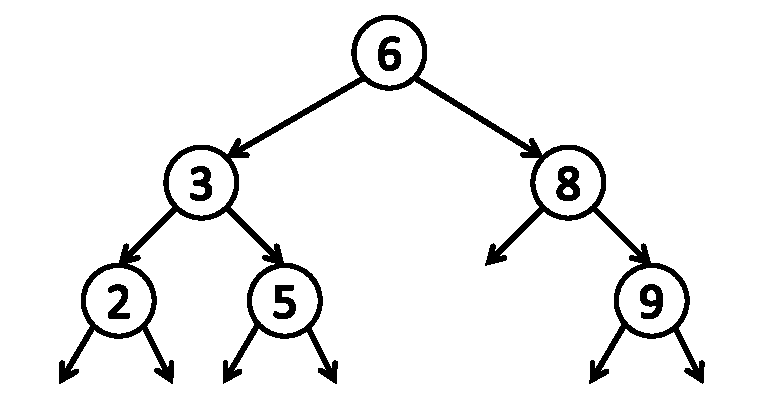
\includegraphics[width=0.5\textwidth]{figureTree.pdf}
%\caption{This is a figure text.}
%\label{fig:ex}
%\end{figure}
\newpage
\thispagestyle{empty}
\mbox{}

\pagebreak
\thispagestyle{empty}
\textbf{Abstract}

abstract goes here


\newpage
\thispagestyle{empty}
\textbf{Acknowledgements}

Acknowledgements goes here


\newpage
\thispagestyle{empty}
\tableofcontents
\pagebreak

\newpage
\thispagestyle{fancyplain}
\section{Introduction}


%  State of high performance computing
%  Shared memory and message passing
%  Role of different programming models/abstractions
%  Data centric computation
%  UPC++



\subsection{Contributions}
A framework for implementing distributed algorithms and applications, created in and for C++, using UPC++, a library that provides PGAS mechanisms for communication. The framework provides an alternate programming model for distributed algorithms, in which a computational task, its data and its communication routines, is represented as a single object. 

% Distribution based on 


\subsection{Outline}
123

\newpage
\section{Background}
%  History + State of distributed computing / high performance computing
%  Message passing vs PGAS
%  Data intensive computing
%  Coupling of Data and processing task -> computation close to data
%  benefits of Abstractions + introduce data/task coupling as a potential abstraction
%  Object oriented high performance computing: object contains data AND task
%  Distributed objects
%  
\subsection{State of High Performance Computing}
Software performance gains from increased frequency in single processing units reached its limits many years ago, and multi-core systems has been prominent in personal computing since. Up until the early 2000s, the speed at which computers could execute sequential programs would steadily increase as clock speed and semiconductor fabrication improved \cite{sutter_larus_2005}. Heat dissipation and energy consumption caused development of the maximum achievable CPU frequency to stall, effectively freezing the number of tasks that can be completed within a certain time frame on a single processing unit \cite{diaz_munoz-caro_nino_2012}. Yet, the size of computational tasks and the amount of data is still increasing, resulting in single-core systems not being able to keep up with the demands of problems found in modern science, engineering and business. 

The answers to these problems were multi-core and many-core systems, which bypasses the aforementioned performance wall by utilizing several processing units. Within the field of high performance computing, however, multi-processor systems were not a novelty. Using networks of workstation computers for parallel computation was an attractive alternative to traditional supercomputers, partly because new processor technology could easily be incorporated without replacing the entire system \cite{wilkinson_allen_2005}. While the field of parallel programming was relevant in high-end scientific applications before halt in clock speed development and the following \emph{concurrency revolution}, homogeneous distributed systems now dominate the field of high performance computing.

Multi-core and many-core architectures achieve parallelism through explicit task distribution and scheduling, managed by the programmer. Exploiting parallelism is often an application-specific issue, and can pose several challenges. In the fields of distributed- and high performance-computing, aiming for scalability further increases the complexity of the programming task. Several programming models have been devised to support development of distributed, parallel applications, and the current leading models can be clustered into different language paradigms: \emph{shared memory }and \emph{message passing} \cite{pgas_languages}.

\subsection{Programming models}
On top of these models, abstractions can be applied to hide complexity from the programmer in order to reduce development time and ease the debugging process. 

There exists a perception that abstraction carry an inherent performance penalty, but abstractions can also be powerful tools in high performance computing \cite{mccandless_lumsdaine_1997}. For example, computing at a large scale can introduce issues relating to handling large amounts of data, scaling to a large or arbitrary number of computation nodes, or developing algorithms that utilizes communication routines and synchronization.

Identifying common patterns in different problems allows for development of frameworks and libraries that are optimized to handle classes of problems matching the same patterns. For example, the MapReduce framework hides significant programming overhead of problems that can be expressed within semantics provided by the framework and the programming model it represents. In its most primitive, data is supplied to the \emph{Map} function and a function to execute on the data is supplied to the \emph{Reduce} function. The MapReduce programming model is designed for algorithms and problems that can be expressed using these two functions, and the MapReduce framework is implemented to provide functionality that can be applied generally to problems within that programming model. In addition to implementing communication routines and data distribution logic, the framework can supply scalability and fault tolerance, due to the information of the application that is implied by the programming model it is utilizing. Other examples of systems specialized in specific programming models include Dryad \cite{dryad}, which models an application's data flow into directed acyclic graphs, and Pregel \cite{pregel}, a framework for graph processing.

\subsection{Data intensive computing}

\subsection{PGAS}
\cite{pgas_upc_energy}

\subsection{GASNet}

\subsection{UPC++}

\newpage
\section{Design}
Saddlebags is a framework for parallel computing, aimed at applications and algorithms that can be implemented in C++. It uses UPC++ for thread spawning, communication, and data distribution, which provides PGAS mechanisms and language constructs such as remote procedure calls, virtual shared memory, and distributed objects. Saddlebags provides a programmer with objects and functions that are inherently distributed, and can be extended with methods and data to express different algorithms.

This section will cover the design and architecture of the system, outlining its different components, its programming model, and data flow. Section 3.1 explains the core concept and design philosophy of Saddlebags, Section 3.2 explains the programming model and data flow, while Section 3.3 outlines the architecture.

\subsection{Motivation}
Saddlebags is designed with several key features in mind, all of them related to what responsibilities a parallel computing framework can take off the an application developer's hands. Some of the underlying concepts and the motivation behind expanding upon the functionality of UPC++ follows.
\\


\hspace{4ex} \textbf{1. Computational tasks should be executed in the same partition in which the data it requires is located}

Problems that can be expressed with data parallelism \cite{data_parallelism} can be distributed across computing units as individual tasks related to specific data. A key concept within PGAS programming is that a private memory segment has affinity to a single computing unit. To exploit data locality, a computational task should only be performed on the unit of computing which the data it requires has affinity to. Expressing behavior like this is trivial when the distribution of data is deterministic. Another wording of the same behavior is that computational tasks have affinity to the data it requires, the same way data has affinity to a computing unit and its private memory segment.
\\

\hspace{4ex} \textbf{2. A multitude of data should be implicitly distributed across available partitions}

Following the principle of a computational task's affinity to its data, full utilization of available processing units is only possible when a program's data is distributed. This means that data used in parallel processing should always be distributed across available memory partitions, so that the computational tasks that require the data is equally distributed.
\\	

\hspace{4ex} \textbf{3. The programmer should not need to write communication routines such as messages or remote procedure calls}

The purpose of building a framework on top of UPC++ is to provide interfaces for the implementation of distributed applications without the complexity of communication routines. While computation methods are application-specific, communication patterns can be implemented for a general case. When claiming that programmers are relieved of writing communication routines, it refers to the need for knowing where data is physically stored, which partition to communicate with, and the need for ensuring that messages are delivered before continuing computation. Data movement will still be explicit, but expressed in an abstraction level in which data locality and memory partitioning is not considered.

Saddlebags presents a programming model that is devised from a specific communication model, and it is assumed that algorithms that can be expressed within this model can also be implemented to communicate in a general pattern. Predictable communication patterns also allows for optimizations and reduces the need for application-specific synchronization. This also makes the physical distribution of data transparent to the programmer.
\\

The goal of building a framework on these specific features is to allow computational parallelism to be expressed with the same semantics as data parallelism, while still allowing tasks to communicate data between each other. The complexity of implementing applications that fit this classification is reduced by utilizing a general communication pattern that relieves programmers of implementing specialized communication. Programmers will in this framework use communication routines by referring to data rather than physical location in the form of partition or computing unit.

\subsection{Programming model}
123123
\subsection{Architecture}
\subsubsection{Item}
\subsubsection{Table}
Distributor
\subsubsection{Worker}


The communication patterns of a push/pull paradigm is simple enough that computational costs of communication in an application can be reasoned about, despite implementation complexity being hidden. 

The Lighght framework is designed with the goal that abstractions provided through C++ mechanisms such as inheritance and type templates should not affect algorithmic complexity: This will only be true for algorithms that can be tailored to the push/pull/work paradigm. 

\newpage
\section{Related work}
\subsection{Husky}
\subsection{Spark}
%% Data MPI?
%% PGAS energy evaluation?

\newpage
\section{Implementation}
\subsection{Distributed objects}
\subsection{Templates}
\subsection{Table}
\subsection{Synchronization}
barriers in cycle
\subsection{Usage}

\newpage
\section{Evaluation}
\subsection{Expressiveness}
\subsection{Energy efficiency}
\subsection{Abstraction costs}
\subsection{Comparison with other systems}

\newpage
\section{Future work}
\subsection{Fault tolerance}
\subsection{View based serialization}

\newpage
\section{Conclusion}



% References. Use IEEE as citation style, and load references from report.bib.
\pagebreak
\bibliographystyle{ieeetr}
\bibliography{report}

% End of document
\end{document}
\grid
\grid
